%label:"con:symplecticCohomology"
%author:JeffHicks
%name:"constructing $\SH(G)$"
%type:"construction"


        %Two Definitions of Symplectic Cohomology
    We now give two different constructions of the symplectic cohomology. In both constructions, it is necessary to deal with the non-compactness of the space $\check X$.
    The first defines the symplectic cohomology as the Floer cohomology of a Hamiltonian whose slope increases along the symplectization coordinate to infinity. The second defines the symplectic cohomology as the limit of Floer cohomology of linear Hamiltonians, where the limit is taken over increasing slopes.
    
    %label:"art:maximumPrinciples"
%author:JeffHicks
%name:"maximum principles"
%type:"exposition"
We recall some of the basics of Hamiltonian Floer theory. Let $X$ be a compact symplectic manifold. 
Given $H_t: X\times \RR\to \RR$ a time dependent Hamiltonian, we obtain an action on the free loop space
%type:equation
%label:eqn:floerAction
%name:"Floer action"


\begin{equation}
    A_{H_t}(\gamma)=-\int_\gamma \lambda + \int_\gamma H_t dt
    \label{eqn:floerAction}
\end{equation}
whose critical points are the time one periodic orbits of $V_{H_t}$. Given a $\omega$-compatible almost complex structure, we observe that cylinders $u: \RR_s\times S^1_t\to X$ which satisfy the $H_t$ perturbed Floer equation
%type:equation
%label:eqn:floerEquation
%name:"Floer equation"


\begin{equation}
    \partial_s u + J(\partial_t u - V_{H_t})=0
    \label{eqn:floerEquation}
\end{equation}
parameterize the negative gradient flow lines of $A_{H_t}$. For curves $\gamma_+, \gamma_-$, let $\mathcal M(\gamma_+, \gamma_-)$ denote the moduli space of solutions to Floer's equation with ends limiting to $\gamma_+, \gamma_-$.
Supposing that $X$ is an exact symplectic manifold, and that our time-dependent Hamiltonian is chosen in a generically, the Floer cochains $\CF(X, H_t)$ are the graded vector space generated  on the time one orbits of $H_t$.
We take a slightly different convention (following Equation 5.2 of \cite{abouzaid2010geometric}) and give each orbit the grading $\deg(\gamma)=n-CZ(\gamma)$, where $CZ(\gamma)$ is the Conley-Zehnder index.
The structure coefficients of the differential are given by counts of solutions to Floer's equation. The theory becomes powerful when it satisfies the following properties:
\begin{itemize}
    \item $\CF(X, H_t)$ is a chain complex. The key step is to show that when $\dim(\mathcal M(\gamma_+, \gamma_-))=1$, there exists a compactification of this moduli space by including broken cylinders. A compactification of the space comes from applying Gromov compactness, while additional requirements on $X$ are sometimes required ensure that the only configurations which appear in the compactification are broken cylinders. In our setting, the only breaking configurations which may occur are broken cylinders, as $X$ is exact (so $\omega(\pi_2(X))=0)$.
    \item Given $H_{t, 0}$ and $H_{t, 1}$ two time-dependent Hamiltonians, there exists a continuation map $\CF(X, H_{t, 0})\to \CF(X, H_{t, 1})$. Furthermore, this map is a homotopy equivalence. 
    \item Finally, we need some way to compute $\CF(X, H_{t, 1})$. One way to do this is to observe that for $C^2$ small Hamiltonians the Floer cochains agree with the Morse cochains (and only consist of constant orbits). By either using the PSS-isomorphism or by analyzing Floer trajectories, the Floer cohomology can be compared to the Morse cohomology of $X$.
\end{itemize}
The major difference in defining the Hamiltonian Floer cohomology for Liouville domains $X$ (as opposed to compact symplectic manifolds) comes from the proof of Gromov-compactness. The first step in the proof of Gromov-compactness is to apply Arzel\'a-Ascoli to out sequence of pseudoholomorphic maps.  Because $\hat X$ is not compact, we cannot apply the Arzel\'a-Ascoli theorem to a sequence of pseudoholomorphic cylinders $u: S^1\times \RR \to \hat X$. 

We now give an example of where we can solve the issue of non-compactness.
%label:"exm:compactnessFromMaximumModulus"
%name:"maximum modulus provides compactness"
%type:"example"



    The maximum modulus principle states that if $\phi: D^2\to \CC$ is a holomorphic function from the disk to $\CC$, that the maximum of $|\phi|: D^2\to \RR_{\geq 0}$ is achieved on $\partial D^2$.

    Let $\hat X$ be a non-compact symplectic manifold with compatible almost complex structure $J$, along with a $J-\jmath$-holomorphic projection $W: \hat X\to \CC$. Suppose that the fibers of $W$ are compact. Pick two loops $\gamma_-, \gamma_+\subset \hat X$ and $r_0\in \RR$ large enough so that $U:=W^{-1}(\{z \st |z|\leq r\})$ contains $\gamma_-, \gamma_+$. We will prove that every pseudoholomorphic cylinder $u: S^1\times \RR\to \hat X$ with ends limiting to $\gamma_-, \gamma_+$ has image contained within the compact subset $U$. 

    The composition $W\circ u: S^1\times \RR\to \CC$ is a holomorphic map, with ends limiting to $W(\gamma_\pm)$, and therefore satisfies the maximum modulus principle. Since the boundary is sent to $W(\gamma_\pm)$, we obtain that $|W|$ achieves a value no greater than $r_0$ on $u$; therefore $\Im(u)\subset U$. It follows that the image of $u$ is contained within a compact set. 
    \label{exm:compactnessFromMaximumModulus}

In order to extend \cref{exm:compactnessFromMaximumModulus} to the setting of $\hat X$, we will use the maximum principle. First, we will need to assume that we have chosen our almost complex structure for $\hat X$ so that the sub-bundle spanned by the vector fields $\partial_r, R$ form an almost complex subspace.
%tag:000K
%label:def:contactTypeACS
%author:JeffHicks
%name:"contact type almost complex structure"
%type:definition

 
    Let $\hat X$ be the completion of a Liouville domain. A choice of almost complex structure for $\hat X$ is \emph{of contact type} if 
    \[d(\exp(r))\circ J = -\alpha.\]
    \label{def:contactTypeACS}
 
We will also need to assume that we have chosen our Hamiltonian so that over the symplectization it only depends on the $r$-coordinate.
For such a contact type almost complex structure and Hamiltonian there exists a version of \cref{exm:compactnessFromMaximumModulus}.
%label:"prp:liouvilleIsGeometricallyBounded"
%author:JeffHicks
%name:"Liouville manifolds are geometrically bounded"
%type:"proposition"

 
   \label{prp:liouvilleIsGeometricallyBounded}
    Let $H: \hat X\to \RR$ be a Hamiltonian which on the symplectization takes the form of $h(\exp(r))$. 
    Let $\gamma_+, \gamma_-$ be time 1 orbits of $V_{H_{t}}$. For a contact type almost complex structure, every solution $u: \RR\times S^1\to \hat X$ of the Floer equation with ends limiting to $\gamma_+, \gamma_-$ has image contained in the subset $\hat X|_{\exp(r)\leq C}$, where $C$ is the maximum value of $\exp(r)$ on the orbits $\gamma_+, \gamma_-$.
 
%label:"prf:liouvilleIsGeometricallyBounded"
%author:JeffHicks
%name:"Liouville manifolds are geometrically bounded"
%type:"proof"
%parent:prp:liouvilleIsGeometricallyBounded
%source:"seidel2006biased"

 
      Let $u: \RR\times S^1\to \RR$ be a solution to the Floer equation (\cref{eqn:floerEquation}). Let $\rho=\exp(r\circ u)$.  By applying $d(\exp(r))$ to the Floer equation, and using \cref{def:contactTypeACS} we obtain :
      \begin{align*}
         0=d(\exp(r))\circ \left(\partial_s u + J(\partial_t u - V_{H})\right)=& \partial_s(\rho) - \alpha(\partial_t u)+ \alpha(V_H)
      \end{align*}
      Because $H= h(\rho)$, the Hamiltonian vector field associated to $H$ is $h'(\rho) V_\alpha$, where $V_\alpha$ is the Reeb flow. From \cref{rem:increasingHamiltonian}, we see that $\alpha(V_H)=h'(\rho).$
      \begin{align*}
         =& \partial_s(\rho) - \alpha(\partial_t u)+ h'(\rho) .
      \end{align*}
      Similarly, applying $\alpha$ to the Floer equation:
      \begin{align*}
         0=\alpha  \left(\partial_s u + J(\partial_t u - V_{H})\right) =& \alpha(\partial_su)+ \partial_t(\exp(\rho))+ V_{H}(\exp(\rho))
         \intertext{Because $H= h(\rho)$ has the same level sets as $\rho$,  $V_H(\rho)=0$. }
         =& \alpha(\partial_s u) + \partial_t(\rho)
      \end{align*}
      Differentiating the first line with respect to $s$,  the second line with respect to $t$, and summing the lines together  we obtain 
      \begin{align*}
        0=&  (\partial_s^2 + \partial_t^2)\circ \rho- \partial_s\alpha(\partial_t u)+\partial_s \rho h'(\rho) +\partial_t\alpha(\partial_s u)\\
        \intertext{As $[\partial_s, \partial_t]=0$, we can substitue $-\partial_t\alpha(\partial_s u)+ \partial_s\alpha (\partial_t u)= -u^*\omega(\partial_s, \partial_t)$ }
        =& \Delta \rho- u^*\omega(\partial_s, \partial_t)+ \rho h'(\rho)\partial_s\rho + \rho h''(\rho) \partial_s\rho\\
        \intertext{By again applying Floer's equation, and using the compatibility of almost complex structure with $J$, we may substitue $u^*\omega(\partial_s, \partial_t)= u^*\omega(\partial_s, J\partial_t-X_H)=|\partial_s u^2|-dh'(\rho)\partial_s$ }
        =& \Delta \rho-|\partial_s|^2+\rho h''(\rho)\partial_s\rho 
      \end{align*}
      We therefore obtain that $\Delta\rho+\rho\cdot h''(\rho) \partial_s\rho\geq 0$. 

      Observe now that where $z\in S^1\times \RR$ is a proposed maximum for $\rho$ that $\partial_s\rho=0$, allowing us to write $(\partial^2_s \rho + \partial^2_t \rho)|_z \geq 0$. This implies that at least one of $\partial^2_s, \partial^2_s$ has to be non-negative --- in particular, the second derivative test does not detect the maximum. A more general argument --- the maximum principle --- states that $\rho$ achieves no local maxima; therefore $\sup_{S^1\times \RR} \rho \leq \max_{t\in S^1} \exp(r\circ \gamma_\pm)=:C.$ It follows that the image of $u$ is contained in $\hat X|_{\rho< C}$, which is a compact set.
 

    
        %tag:000X
%label:"con:symplecticCohomologyQuadratic"
%author:JeffHicks
%name:"$\SH(X)$ via quadratic $H$"
%type:"construction"


   \label{con:symplecticCohomologyQuadratic}
   Let $(X, \lambda)$ be a Liouville domain, and let $\hat X$ be its completion. The goal is to construct a Floer cohomology which witnesses all of the Reeb orbits of $\partial X$. With that in mind, it is natural to study the Hamiltonian Floer cohomology of Hamiltonians $H_t$ with the property that over the symplectization they are of the form 
   \[H|_{\RR\times \partial X}=h(\exp(r))\]
   where $\lim_{r\to\infty} h'(\exp(r))=\infty$. This Hamiltonian witnesses every Reeb orbit with sufficiently large period. 
   %label:"fig:quadraticHamiltonian"
%author:JeffHicks
%name:"quadratic Hamiltonian"
%type:"figure"
%parent:con:symplecticCohomologyQuadratic
%caption:"An increasing Hamiltonian over the symplectization witnesses all Reeb orbits"


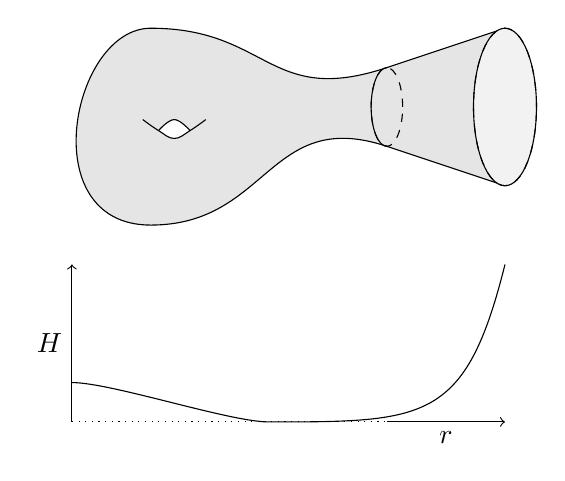
\begin{tikzpicture}
    \draw[fill=gray!20] (4,-0.5) .. controls (2.5,-1) and (4,-0.5) .. (2.5,-1) .. controls (1,-1.5) and (1,-0.5) .. (-0.5,-0.5) .. controls (-1.5,-0.5) and (-2,-3) .. (-0.5,-3) .. controls (1,-3) and (1,-1.5) .. (2.5,-2) .. controls (4,-2.5) and (2.5,-2) .. (4,-2.5);
    \begin{scope}[shift={(3.2,-2)}]
    
    \fill[white]  plot[smooth, tension=0.7] coordinates { (-3.6,0.2) (-3.4,0.1) (-3.2,0.2) }  plot[smooth, tension=0.7] coordinates {(-3.6,0.2) (-3.4,0.34) (-3.2,0.2)};
    
    \draw  plot[smooth, tension=0.7] coordinates {(-3.8,0.34) (-3.6,0.2) (-3.4,0.1) (-3.2,0.2) (-3,0.34)};
    \draw  plot[smooth, tension=0.7] coordinates {(-3.6,0.2) (-3.4,0.34) (-3.2,0.2)};
    
    
    
    \end{scope}
    
    \begin{scope}[]
    
    \draw[dashed]  (2.5,-1.5) ellipse (0.2 and 0.5);
    \clip  (2,-1) rectangle (2.5,-2);
    
    \draw  (2.5,-1.5) ellipse (0.2 and 0.5);
    \end{scope}
    
    \begin{scope}[scale=2, shift={(-0.5,0.75)}]
    
    \draw[dashed, fill=gray!10]  (2.5,-1.5) ellipse (0.2 and 0.5);
    
    
    \draw  (2.5,-1.5) ellipse (0.2 and 0.5);
    \end{scope}
    
    \draw[dotted] (-1.5,-5.5) -- (2.5,-5.5);
    \draw[->] (2.5,-5.5) --node[below]{$r$} (4,-5.5);
    \draw (-1.5,-5) .. controls (-1,-5) and (0.5,-5.5) .. (1,-5.5) .. controls (3,-5.5) and (3.5,-5.5) .. (4,-3.5);
    
    \draw[->] (-1.5,-5.5) -- node[left]{$H$} (-1.5,-3.5);
    \end{tikzpicture}
   
   A problem with this definition is that the Hamiltonian we have chosen is time independent, and so whenever $(\partial X, \alpha)$ has any Reeb orbits, the time-1 orbits of $H$ will necessarily be degenerate (all orbits come in $S^1$ families from reparameterization). The standard work-around is to introduce a small time-dependent perturbation to $H$ in such a way that we can still apply our maximum principle argument. We therefore look at time-dependent Hamiltonians $H_t$ which, outside of a compact set, are of the form $h_t(\exp(r))$, with $\lim_{r\to\infty} h_t(\exp(r))=\infty$ for all $t$. The maximum principle argument from \cref{prp:liouvilleIsGeometricallyBounded} can be made to hold in this setting (Proposition 4.1 \cite{wendlbeginner}).

   One then takes the definition of the symplectic cohomology to be 
   \[\SH(X):=\CF(\hat X, H_t)=\bigoplus_{\gamma\;|\; \dot \gamma= V_{H_t}} \ZZ\langle \gamma\rangle.\]
   with differential given by structure coefficients $\langle d(\gamma_+), \gamma_\rangle$ counting $V_{H_t}$-perturbed pseudoholomorphic cylinders with ends limiting to $\gamma_\pm$.

        %label:"con:symplecticCohomologyLimit"
%author:JeffHicks
%name:"$\SH(X)$ as a limit"
%type:"construction"


    As before, let $(X, \lambda)$ be a Liouville domain. For $m\not\in \ell(\Gamma)$ not a period of a Reeb orbit, define 
    \[\SH(X)^{< m}:=\HF(\hat X, H^m_t)\]
    where $H^m_t$ is a Hamiltonian which on the symplectization agrees with $H^m$, the linear Hamiltonian of slope $m$. 
    Over the symplectization $\RR\times \partial X$ there are no Hamiltonian orbits, as $H^m$ has no Hamiltonian orbits. The $< m$ signifies that this version of symplectic cohomology is only supposed to detect those Reeb orbits of period less than $m$.

    In order to recover the symplectic cohomology, we would like to understand the limit of the groups $SH(X)^{< m}$ as we take $m\to\infty$. Making sense of a limit algebraically requires constructing maps between these groups. When $m^+< m^-$, the maximum principle arguments applied to families of Hamiltonians dependent on the $s$-parameter hold, allowing us to construct chain maps 
    \[\CF(\hat X, H^{m^+}_t)\to \CF(\hat X, H^{m^-}_t)\]
    The $\pm$ index on the slope are meant to represent whether they are the incoming or outgoing side of a Floer trajectory, not the relative sizes of the slopes. From the perspective of \cref{con:symplecticCohomologyQuadratic}, the set of Hamiltonian orbits corresponding to Reeb orbits of period less than $m^+$ is a subcomplex of the set of Reeb orbits of period less than $m^-$. Intuitively, the Floer trajectory should decrease the action associated to the Reeb vector field, which is the period of the Reeb orbit.
    %label:"fig:limitHamiltonian"
%author:JeffHicks
%name:"limit Hamiltonian"
%type:"figure"
%parent:"con:symplecticCohomologyLimit"
%caption:"A limit of Hamiltonians of increasing slopes eventually sees all Reeb orbits"

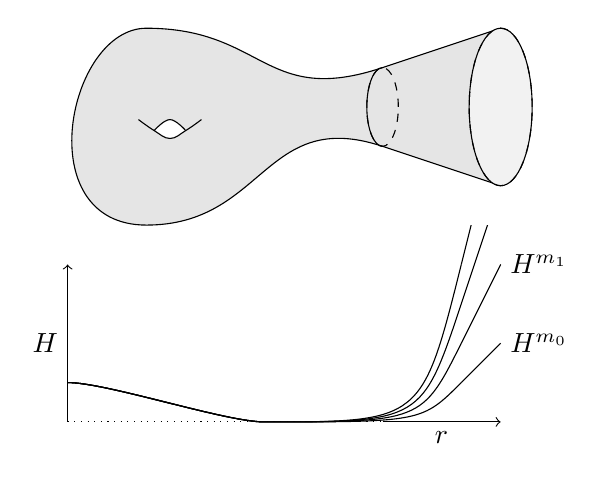
\begin{tikzpicture}
    \draw[fill=gray!20] (4,-0.5) .. controls (2.5,-1) and (4,-0.5) .. (2.5,-1) .. controls (1,-1.5) and (1,-0.5) .. (-0.5,-0.5) .. controls (-1.5,-0.5) and (-2,-3) .. (-0.5,-3) .. controls (1,-3) and (1,-1.5) .. (2.5,-2) .. controls (4,-2.5) and (2.5,-2) .. (4,-2.5);
    \begin{scope}[shift={(3.2,-2)}]
    
    \fill[white]  plot[smooth, tension=0.7] coordinates { (-3.6,0.2) (-3.4,0.1) (-3.2,0.2) }  plot[smooth, tension=0.7] coordinates {(-3.6,0.2) (-3.4,0.34) (-3.2,0.2)};
    
    \draw  plot[smooth, tension=0.7] coordinates {(-3.8,0.34) (-3.6,0.2) (-3.4,0.1) (-3.2,0.2) (-3,0.34)};
    \draw  plot[smooth, tension=0.7] coordinates {(-3.6,0.2) (-3.4,0.34) (-3.2,0.2)};
    
    
    
    \end{scope}
    
    \begin{scope}[]
    
    \draw[dashed]  (2.5,-1.5) ellipse (0.2 and 0.5);
    \clip  (2,-1) rectangle (2.5,-2);
    
    \draw  (2.5,-1.5) ellipse (0.2 and 0.5);
    \end{scope}
    
    \begin{scope}[scale=2, shift={(-0.5,0.75)}]
    
    \draw[dashed, fill=gray!10]  (2.5,-1.5) ellipse (0.2 and 0.5);
    
    
    \draw  (2.5,-1.5) ellipse (0.2 and 0.5);
    \end{scope}
    \clip  (5,-6) rectangle (-2,-3);
    \draw[dotted] (-1.5,-5.5) -- (2.5,-5.5);
    \draw[->] (2.5,-5.5) --node[below]{$r$} (4,-5.5);
    \draw (-1.5,-5) .. controls (-1,-5) and (0.5,-5.5) .. (1,-5.5) .. controls (3,-5.5) and (3,-5.5) .. (3.5,-5);
    \draw (-1.5,-5) .. controls (-1,-5) and (0.5,-5.5) .. (1,-5.5) .. controls (3,-5.5) and (3,-5.5) .. (3.5,-3.5);
    \draw (-1.5,-5) .. controls (-1,-5) and (0.5,-5.5) .. (1,-5.5) .. controls (3,-5.5) and (3,-5.5) .. (3.5,-4);
    \draw (-1.5,-5) .. controls (-1,-5) and (0.5,-5.5) .. (1,-5.5) .. controls (3,-5.5) and (3,-5.5) .. (3.5,-4.5);
    
    \draw[->] (-1.5,-5.5) -- node[left]{$H$} (-1.5,-3.5);
    \draw (3.5,-5) -- (4,-4.5) (3.5,-4.5) -- (4,-3.5) (3.5,-4) -- (4,-2.5) (3.5,-3.5) -- (4,-1.5);
    
    \node[right] at (4,-4.5) {$H^{m_0}$};
    \node[right] at (4,-3.5) {$H^{m_1}$};
    \node[right] at (4,-2.5) {$\vdots$};
    \end{tikzpicture}

    Consider now an increasing sequence of slopes $m_0< m_1< \cdots $ which are not the periods of any Reeb orbits of $\partial X$. One can form the telescope complex
    \input{dig_symplenicticCohomologyTelescope}
    where the vertical maps are the identity, and the diagonal maps are continuations.
    %label:"prp:homologyOfTelescope"
%author:JeffHicks
%name:"homology of telescope complex"
%type:"proposition"


    The cohomology of the telescope complex $\bigoplus_{i=0}^\infty C^\bullet_i \oplus C^\bullet_{i-1}$ is $\lim_{i\to\infty} H(C^\bullet_i)$.
 
    We could therefore also define
    \[SH(X):=\lim_{i\to\infty} \SH(X)^{< m^i}.\]

        %label:"art:algebraicStructuresOnSH"
%author:JeffHicks
%name:"ring structure on $\SH(X)$"
%type:"article"

Without proof, we describe some of the algebraic structures on the symplectic cohomology. 

First, the construction of the pair of pants product on Hamiltonian Floer cohomology can be extended to give a pair-of-pants product on the symplectic cohomology. This makes $\SH(X)$ into a graded ring. Furthermore, the symplectic cohomology is a ring with unit.


